% SPDX-License-Identifier: CC-BY-SA-4.0
%
% Copyright (c) 2020 Philipp Le
%
% Except where otherwise noted, this work is licensed under a
% Creative Commons Attribution-ShareAlike 4.0 License.
%
% Please find the full copy of the licence at:
% https://creativecommons.org/licenses/by-sa/4.0/legalcode

\chapter{Sampling and Time-Discrete Signals and Systems}

\begin{refsection}

\section{Time-Discrete Signals}

\subsection{Ideal Sampling}

\begin{figure}[H]
	\centering
	\begin{tikzpicture}
		\begin{axis}[
			height={0.25\textheight},
			width=0.6\linewidth,
			scale only axis,
			xlabel={$t$},
			ylabel={$x$},
			%grid style={line width=.6pt, color=lightgray},
			%grid=both,
			grid=none,
			legend pos=north west,
			axis y line=middle,
			axis x line=middle,
			every axis x label/.style={
				at={(ticklabel* cs:1.05)},
				anchor=north,
			},
			every axis y label/.style={
				at={(ticklabel* cs:1.05)},
				anchor=east,
			},
			%xmin=0,
			%xmax=7,
			%ymin=0,
			%ymax=3,
			%xtick={0, 1, ..., 6},
			%ytick={0, 0.5, ..., 2.5},
			xmin=0,
			xmax=6.5,
			xtick={0, 1, ..., 6},
			xticklabels={$0$, $T_S$, $2 T_S$, $3 T_S$, $4 T_S$, $5 T_S$, $6 T_S$},
		]
			\addplot[smooth, blue, dashed] coordinates {(0, 1.1) (1, 1.8) (2, 2.1) (3, 1.0) (4, 0.8) (5, 1.7) (6, 2.4)};
			\addlegendentry{$\underline{x}{t}$};
			\addplot[red, thick] coordinates {(0, 0) (0, 1.1)};
			\addplot[red, thick] coordinates {(1, 0) (1, 1.8)};
			\addplot[red, thick] coordinates {(2, 0) (2, 2.1)};
			\addplot[red, thick] coordinates {(3, 0) (3, 1.0)};
			\addplot[red, thick] coordinates {(4, 0) (4, 0.8)};
			\addplot[red, thick] coordinates {(5, 0) (5, 1.7)};
			\addplot[red, thick] coordinates {(6, 0) (6, 2.4)};
			\addplot[only marks, red, thick, mark=o] coordinates {(0, 1.1) (1, 1.8) (2, 2.1) (3, 1.0) (4, 0.8) (5, 1.7) (6, 2.4)};
			\addlegendentry{$\underline{x}_S{t}$};
		\end{axis}
	\end{tikzpicture}
	\caption{Sampling of a time-continuous signal}
	\label{fig:ch04:sampling_of_signal}
\end{figure}

Sampling:
\begin{itemize}
	\item Sampling is converting a time-continuous signal $\underline{x}(t)$ to a time-discrete signal $\underline{x}[n]$.
	\item Samples are periodically taken out of the original signal.
\end{itemize}

Nomenclature:
\begin{itemize}
	\item The original time-continuous signal is $\underline{x}(t)$. The continuous time variable $t \in \mathbb{R}$ is a continuous real number.
	\item The sampled signal is $\underline{x}[n]$. The discrete time variable $n \in \mathbb{Z}$ is a (discrete) integer number.
	\item Round parenthesis is used for time-continuous signals. Square parenthesis is used for time-discrete signals.
\end{itemize}

Sampling parameters:
\begin{itemize}
	\item The time instances, at which the samples are taken out, are equidistant.
	\item The period between the samples is the \index{sampling period} \textbf{sampling period} $T_S$.
	\item The inverse of the sampling period is the \index{sampling rate} \textbf{sampling rate} $f_S$.
	\begin{equation}
		f_S = \frac{1}{T_S}
	\end{equation}
	\item The \index{sampling angular frequency} \textbf{sampling angular frequency} $\omega_S$.
	\begin{equation}
		\omega_S = \frac{2 \pi}{T_S}
	\end{equation}
\end{itemize}

Ideal sampling:
\begin{itemize}
	\item The samples are ideally equidistant. The sampling period $T_S$ is constant and is \underline{not} subject to fluctuations.
	\item The sample has the value of the original signal $\underline{x}(t)$ at \underline{exactly} the time instance where has been taken.
\end{itemize}
Some corollaries can be deducted from these two points:
\begin{itemize}
	\item The sampled signal $\underline{x}_S(n T_S)$ at the discrete time $n$ is the value of the original signal at time $t = n T_S$.
	\begin{equation}
		\underline{x}[n] = \underline{x}\left(n T_S\right)
	\end{equation}
	\item The sampled signal $\underline{x}_S(t)$ consists of a chain of equidistant, indefinitely narrow pulses.
	\begin{itemize}
		\item The pulses are equidistant with $T_S$.
		\item The pulses have the value of $\underline{x}\left(n T_S\right)$ as their amplitudes.
		\item The value of the sampled signal is zero in between the pulses.
		\begin{equation}
			\underline{x}_S(t) = \begin{cases}
				\underline{x}\left(n T_S\right) & \quad \forall \; t = n T_S, n \in \mathbb{Z}, \\
				0 & \quad \forall \; n T_S < t < \left(n+1\right) T_S, n \in \mathbb{Z}.
			\end{cases}
		\end{equation}
	\end{itemize}
\end{itemize}

\subsubsection{Dirac comb}

We know already indefinitely narrow pulses. They are Dirac delta functions $\delta\left(t - n T_S\right)$.

Taking out \underline{exactly one} sample out of $\underline{x}(t)$ is a multiplication of $\underline{x}(t)$ with $\delta\left(t - n T_S\right)$.
\begin{equation}
	\underline{x}_{S,n}(t) = \underline{x}(t) \delta\left(t - n T_S\right)
	\label{eq:ch4:one_sample_1}
\end{equation}
The Dirac delta function is zero expect at $t = n T_S$. So, \eqref{eq:ch4:one_sample_1} can be further reduced.
\begin{equation}
	\underline{x}_{S,n}(t) = \underline{x}(n T_S) \delta\left(t - n T_S\right)
	\label{eq:ch4:one_sample_2}
\end{equation}

\begin{figure}[H]
	\centering
	\begin{tikzpicture}
		\begin{axis}[
			height={0.25\textheight},
			width=0.6\linewidth,
			scale only axis,
			xlabel={$t$},
			ylabel={$x$},
			%grid style={line width=.6pt, color=lightgray},
			%grid=both,
			grid=none,
			legend pos=north west,
			axis y line=middle,
			axis x line=middle,
			every axis x label/.style={
				at={(ticklabel* cs:1.05)},
				anchor=north,
			},
			every axis y label/.style={
				at={(ticklabel* cs:1.05)},
				anchor=east,
			},
			%xmin=0,
			%xmax=7,
			%ymin=0,
			%ymax=3,
			%xtick={0, 1, ..., 6},
			%ytick={0, 0.5, ..., 2.5},
			xmin=0,
			xmax=6.5,
			xtick={0, 1, ..., 6},
			xticklabels={$0$, $T_S$, $2 T_S$, $3 T_S$, $4 T_S$, $5 T_S$, $6 T_S$},
		]
			\addplot[smooth, blue, dashed] coordinates {(0, 1.1) (1, 1.8) (2, 2.1) (3, 1.0) (4, 0.8) (5, 1.7) (6, 2.4)};
			\addlegendentry{$\underline{x}{t}$};
			\addplot[red, thick] coordinates {(2, 0) (2, 2.1)};
			\addplot[only marks, red, thick, mark=o] coordinates {(2, 2.1)};
			\addlegendentry{$\underline{x}_{S,n}{t}$};
		\end{axis}
	\end{tikzpicture}
	\caption[Taking out exactly one sample out of $\underline{x}(t)$]{Taking out exactly one sample out of $\underline{x}(t)$ -- in this example $n = 2$.}
\end{figure}

To obtain the sampled signal, the sampling process $\underline{x}_{S,n}(t)$ \eqref{eq:ch4:one_sample_1} needs to be repeated for each $n \in \mathbb{Z}$. All individual sample processes $\underline{x}_{S,n}(t)$ are then superimposed to form the complete sampled signal $\underline{x}_S(t)$.
\begin{equation}
	\begin{split}
		\underline{x}_S(t) &= \sum\limits_{n = -\infty}^{\infty} \underline{x}_{S,n}(t) \\
		 &= \sum\limits_{n = -\infty}^{\infty} \underline{x}\left(t\right) \delta\left(t - n T_S\right) \\
		 &= \underline{x}\left(t\right) \cdot \underbrace{\sum\limits_{n = -\infty}^{\infty} \delta\left(t - n T_S\right)}_{= \Sha_{T_S}(t)}
	\end{split}
\end{equation}

The sum of Dirac delta functions
\begin{itemize}
	\item forms a series of equidistant pulses repeating at a period of $T_S$,
	\item is called \index{Dirac comb} \textbf{Dirac comb} $\Sha_{T_S}(t)$ or \index{impulse train} \textbf{impulse train}.
\end{itemize}

\begin{definition}{Dirac comb}
	The \index{Dirac comb} \textbf{Dirac comb} $\Sha_{T}(t)$ or \index{impulse train} \textbf{impulse train} is:
	\begin{equation}
		\Sha_{T}(t) = \sum\limits_{n = -\infty}^{\infty} \delta\left(t - n T\right)
		\label{eq:ch04:dirac_comb}
	\end{equation}
	$T$ is the period of the equidistant Dirac pulses.
	
	It is a periodic signal and can be decomposed using the Fourier analysis:
	\begin{equation}
		\Sha_{T}(t) = \frac{1}{T} \sum\limits_{n = -\infty}^{\infty} e^{j n \frac{2 \pi}{T} t}
		\label{eq:ch04:dirac_comb_fourier_series}
	\end{equation}
	
	\begin{figure}[H]
		\centering
		\begin{tikzpicture}
			\begin{axis}[
				height={0.15\textheight},
				width=0.9\linewidth,
				scale only axis,
				xlabel={$t$},
				ylabel={$\Sha_{T_S}(t)$},
				%grid style={line width=.6pt, color=lightgray},
				%grid=both,
				grid=none,
				legend pos=north east,
				axis y line=middle,
				axis x line=middle,
				every axis x label/.style={
					at={(ticklabel* cs:1.05)},
					anchor=north,
				},
				every axis y label/.style={
					at={(ticklabel* cs:1.05)},
					anchor=east,
				},
				xmin=-5.5,
				xmax=5.5,
				ymin=0,
				ymax=1.2,
				xtick={-5, -4, ..., 5},
				xticklabels={$-5 T_S$, $-4 T_S$, $-3 T_S$, $-2 T_S$, $- T_S$, $0$, $T_S$, $2 T_S$, $3 T_S$, $4 T_S$, $5 T_S$},
				ytick={0},
			]
				\pgfplotsinvokeforeach{-5, -4, ..., 5}{
					\draw[-latex, blue, very thick] (axis cs:#1,0) -- (axis cs:#1,1);
					%\addplot[blue, very thick] coordinates {(#1, 0) (#1, 1)};
					%\addplot[only marks, blue, thick, mark=triangle] coordinates {(#1, 1)};
				}
			\end{axis}
		\end{tikzpicture}
		\caption{Dirac comb}
	\end{figure}
\end{definition}

\subsubsection{Ideal Sampler}

A \index{sampler} \textbf{sampler} is a system which
\begin{itemize}
	\item applies the Dirac comb $\Sha_{T_S}(t)$
	\item to a time-continuous signal $\underline{x}(t)$ (multiplication) and
	\item outputs a series of equidistant pulses $\underline{x}_S(t)$.
\end{itemize}

\begin{definition}{Ideally sampled signal}
	An ideally \index{sampled signal} sampled signal is:
	\begin{equation}
		\begin{split}
			\underline{x}_S(t) &= \underline{x}(t) \cdot \Sha_{T_S}(t) \\
			 &= \sum\limits_{n = -\infty}^{\infty} \underline{x}\left(t\right) \delta\left(t - n T_S\right) \\
			 &= \sum\limits_{n = -\infty}^{\infty} \underline{x}\left(n T_S\right) \delta\left(t - n T_S\right)
		\end{split}
		\label{eq:ch04:ideal_sampling}
	\end{equation}
\end{definition}

The sampled signal $\underline{x}_S(t)$ is a chain of pulses (red signal in Figure \ref{fig:ch04:sampling_of_signal}). The chain of pulses can then be reinterpreted as a time-discrete signal $\underline{x}[n]$. The value of $\underline{x}[n]$ is:
\begin{equation}
	\underline{x}[n] = T_S \underline{x}_S\left(n T_S\right) = \underline{x}\left(n T_S\right) \qquad \forall \; n \in \mathbb{Z}
	\label{eq:ch04:sample_value}
\end{equation}

\begin{figure}[H]
	\centering
	\begin{adjustbox}{scale=0.8}
		\begin{tikzpicture}
			\node[draw, block] (Sampler) {Ideal sampler};
			\node[draw, block, right=3cm of Sampler] (ReInterp) {Reinterpret as\\ time-discrete signal};
			
			\draw[<-o] (Sampler.west) -- ++(-1.7cm, 0) node[above, align=center]{Time-continuous\\ signal $\underline{x}(t)$};
			\draw[->] (Sampler.east) -- (ReInterp.west) node[midway, above, align=center]{Series of pulses\\ $\underline{x}_S(t)$};
			\draw[<-] (Sampler.south) -- ++(0, -0.75cm) node[below, align=center]{Dirac comb\\ $\Sha_{T_S}(t)$};
			\draw[->] (ReInterp.east) -- ++(1.5cm, 0) node[above, align=center]{Time-discrete\\ signal $\underline{x}[n]$};
			
			\draw[dashed] (ReInterp.north) -- ++(0, 2cm) node[below left, align=right]{Time-continuous\\ domain} node[below right, align=left]{Time-discrete\\ domain};
			\draw[dashed] (ReInterp.south) -- ++(0, -1cm);
		\end{tikzpicture}
	\end{adjustbox}
	\caption{An abstract view on sampling}
\end{figure}

\begin{excursus}{Normalisation of the sampled signal}
	\label{ref:ch04:normalization_xs}
	
	You may wonder about the equation \eqref{eq:ch04:sample_value}. Where does the $T_S$ in $T_S \underline{x}_S\left(n T_S\right)$ come from?
	
	\vspace{0.5em}
	
	The value of the sampled signal $\underline{x}_S\left(n T_S\right)$ is normalized by $\frac{1}{T_S}$. This is a result of the normalization of the Dirac delta function. Its argument shall be unitless. However, its argument $t - n T_S$ is a time unit. Consequently, the argument must be normalized by $T_S$.
	\begin{equation}
		\delta\left(t - n T_S\right) = \frac{1}{T_S} \delta\left(\frac{t}{T_S} - n\right)
	\end{equation}
	using the scaling property of the Dirac delta function, which is:
	\begin{equation}
		\delta\left(t\right) = \frac{1}{|a|} \left(\frac{t}{a}\right)
	\end{equation}
	\eqref{eq:ch04:ideal_sampling} can be rewritten to
	\begin{equation}
		\begin{split}
			\underline{x}_S(t) &= \sum\limits_{n = -\infty}^{\infty} \underline{x}\left(n T_S\right) \delta\left(t - n T_S\right) \\
			 &= \sum\limits_{n = -\infty}^{\infty} \underline{x}\left(n T_S\right) \cdot \frac{1}{T_S} \delta\left(\frac{t}{T_S} - n\right) \\
			T_S \underline{x}_S(t) &= \sum\limits_{n = -\infty}^{\infty} \underline{x}\left(n T_S\right) \delta\left(\frac{t}{T_S} - n\right) \\
		\end{split}
	\end{equation}
	The reason why $\underline{x}_S(t)$ needs to be normalized is, that it is an indefinitely small Dirac delta pulse. $T_S$ is the equidistant spacing between the pulses. $\frac{t}{T_S}$ guarantees a normalized spacing of $1$ between the samples.
	
	\vspace{0.5em}
	
	Why is $\underline{x}[n]$ not scaled? It is, but its normalization constant is not explicitly written. The equidistant spacing between $\underline{x}[n]$ and $\underline{x}[n+1]$ is $1$. Thus, their normalization constant is $1$, too.
	\begin{equation*}
		1 \cdot \underline{x}[n] = T_S \underline{x}_S\left(n T_S\right) = \underline{x}\left(n T_S\right)
	\end{equation*}
\end{excursus}

\subsubsection{Irreversibility of Sampling}

\begin{fact}
	The act of sampling is irreversible.
\end{fact}
	
There is a way to obtain the sampled signal:
\begin{equation*}
	\underline{x}_S(t) = \mathrm{Sampling} \left(\underline{x}(t)\right)
\end{equation*}
But there is generally no way back to reconstruct the original signal. $\mathrm{Sampling}^{-1} \left(\underline{x}_S(t)\right)$ does not exist.
\begin{equation*}
	\underline{x}(t) \neq \underbrace{\mathrm{Sampling}^{-1}}_{\text{Does not exist}} \left(\underline{x}_S(t)\right)
\end{equation*}

Sampling is always lossy in general.

\subsection{Sampling Theorem, Aliasing and Reconstruction}

\subsubsection{Frequency Domain Representation}

\begin{excursus}{Fourier transform of the Dirac comb}
	The Fourier transform of the Dirac comb is again a Dirac comb:
	\begin{equation}
		\begin{split}
			\Sha_{T}(t) \TransformHoriz \mathcal{F}\left\{\Sha_{T}(t)\right\} &= \frac{2 \pi}{T} \Sha_{\frac{2 \pi}{T}}(\omega) \\
			 &= \frac{2 \pi}{T} \sum\limits_{k = -\infty}^{\infty} \delta\left(\omega - k \frac{2 \pi}{T}\right) \\
			 &= \sum\limits_{k = -\infty}^{\infty} e^{- j \omega k T}
		\end{split}
		\label{eq:ch04:dirac_comb_fourier_tranform}
	\end{equation}
\end{excursus}

\eqref{eq:ch04:ideal_sampling} pointed out, that the sampled signal $\underline{x}_S(t)$ is the multiplication of the original time-domain signal $\underline{x}(t)$ and the Dirac comb $\Sha_{T_S}(t)$ with a periodicity of the sampling period $T_S$.
\begin{equation}
	\begin{split}
		\underline{x}_S(t) &= \underline{x}(t) \cdot \Sha_{T_S}(t) \\
		 &= \underline{x}(t) \cdot \frac{1}{T_S} \sum\limits_{n = -\infty}^{\infty} e^{j n \frac{2 \pi}{T_S} t} \\
		 &= \frac{1}{T_S} \sum\limits_{n = -\infty}^{\infty} \underbrace{\underline{x}(t) e^{j n \frac{2 \pi}{T_S} t}}_{\text{Frequency shift by } n \frac{2 \pi}{T_S}} \\
	\end{split}
\end{equation}

\textit{Remark:} Please note the normalization of the sampled signal by $T_S$, as explained on page \pageref{ref:ch04:normalization_xs}.

The ideally sampled signal $\underline{x}_S(t)$ can be expressed as a sum of \emph{frequency shifts} of the original signal $\underline{x}(t)$. Its Fourier transform is:
\begin{equation}
	\begin{split}
		\underline{X}_S\left(j \omega\right) &= \mathcal{F}\left\{\frac{1}{T_S} \sum\limits_{k = -\infty}^{\infty} \underline{x}(t) e^{j k \frac{2 \pi}{T_S} t}\right\} \\
		 & \qquad \text{Using the linearity of the Fourier transform:} \\
		 &= \frac{1}{T_S} \sum\limits_{k = -\infty}^{\infty} \mathcal{F}\left\{\underline{x}(t) e^{j k \frac{2 \pi}{T_S} t}\right\} \\
		 & \qquad \text{Using the frequency shift theorem of the Fourier transform:} \\
		 &= \frac{1}{T_S} \sum\limits_{k = -\infty}^{\infty} \underline{X}\left(j \left(\omega - k \frac{2 \pi}{T_S} \right)\right)
	\end{split}
\end{equation}

\textit{Remark:} Please note the normalization of the sampled signal by $T_S$, as explained on page \pageref{ref:ch04:normalization_xs}.

\begin{proof}{}
	An alternative way is using the Fourier transform of this multiplication in the time-domain is a convolution in the frequency domain:
	\begin{equation}
		\begin{split}
			\underline{X}_S\left(j \omega\right) &= \mathcal{F}\left\{\underline{x}(t) \cdot \Sha_{T_S}(t)\right\} \\
			 &= \frac{1}{2 \pi} \underline{X}\left(j \omega\right) * \left(\frac{2 \pi}{T_S} \Sha_{\frac{2 \pi}{T_S}}(\omega)\right) \\
			 &= \frac{1}{T_S} \int\limits_{-\infty}^{\infty} \underline{X}\left(j \left(\omega - \zeta\right)\right) \Sha_{\frac{2 \pi}{T_S}}\left(\zeta\right) \, \mathrm{d} \zeta \\
			 &= \frac{1}{T_S} \int\limits_{-\infty}^{\infty} \underline{X}\left(j \left(\omega - \zeta\right)\right) \sum\limits_{k = -\infty}^{\infty} \delta\left(\zeta - k \frac{2 \pi}{T_S}\right) \, \mathrm{d} \zeta \\
			 &= \frac{1}{T_S} \sum\limits_{k = -\infty}^{\infty} \int\limits_{-\infty}^{\infty} \underline{X}\left(j \left(\omega - \zeta\right)\right) \delta\left(\zeta - k \frac{2 \pi}{T_S}\right) \, \mathrm{d} \zeta \\
			 & \qquad \text{Using the Dirac measure:} \\
			 &= \frac{1}{T_S} \sum\limits_{k = -\infty}^{\infty} \underline{X}\left(j \left(\omega - k \frac{2 \pi}{T_S}\right)\right) \\
		\end{split}
	\end{equation}
\end{proof}

\textbf{Conclusion:} The spectrum of the sampled signal $\underline{X}_S\left(j \omega\right)$
\begin{itemize}
	\item consists of superimposed, frequency-shifted copies of the spectra of the original signal $\underline{X}\left(j\omega\right)$ and
	\item the periodicity of the superimposed, frequency-shifted copies is the sampling angular frequency $\omega_S = \frac{2 \pi}{T_S}$ or sampling frequency $f_S$, respectively,
	\item each frequency-shifted copy starts at $k \omega_S - \frac{\omega_S}{2}$ and ends at $k \omega_S + \frac{\omega_S}{2}$.
\end{itemize}

\begin{figure}[H]
	\subfloat[Original signal $\underline{X}\left(j\omega\right)$] {
		\centering
		\begin{tikzpicture}
				\begin{axis}[
				height={0.15\textheight},
				width=0.9\linewidth,
				scale only axis,
				xlabel={$\omega$},
				ylabel={$|\underline{X}\left(j\omega\right)|$},
				%grid style={line width=.6pt, color=lightgray},
				%grid=both,
				grid=none,
				legend pos=north east,
				axis y line=middle,
				axis x line=middle,
				every axis x label/.style={
					at={(ticklabel* cs:1.05)},
					anchor=north,
				},
				every axis y label/.style={
					at={(ticklabel* cs:1.05)},
					anchor=east,
				},
				xmin=-3.5,
				xmax=3.5,
				ymin=0,
				ymax=1.2,
				xtick={-1, -0.5, 0, 0.5, 1},
				xticklabels={$- \omega_S$, $- \frac{\omega_S}{2}$, $0$, $\frac{\omega_S}{2}$, $\omega_S$},
				ytick={0},
			]
				\draw[green, thick] (axis cs:-0.4,0) -- (axis cs:0,0.7);
				\draw[red, thick] (axis cs:0,0.7) -- (axis cs:0.4,0);
			\end{axis}
		\end{tikzpicture}
	}

	\subfloat[Spectrum of the Dirac comb $\frac{2 \pi}{T} \Sha_{\frac{2 \pi}{T}}(\omega)$] {
		\centering
		\begin{tikzpicture}
			\begin{axis}[
				height={0.15\textheight},
				width=0.9\linewidth,
				scale only axis,
				xlabel={$t$},
				ylabel={$|\frac{2 \pi}{T} \Sha_{\frac{2 \pi}{T}}(\omega)|$},
				%grid style={line width=.6pt, color=lightgray},
				%grid=both,
				grid=none,
				legend pos=north east,
				axis y line=middle,
				axis x line=middle,
				every axis x label/.style={
					at={(ticklabel* cs:1.05)},
					anchor=north,
				},
				every axis y label/.style={
					at={(ticklabel* cs:1.05)},
					anchor=east,
				},
				xmin=-3.5,
				xmax=3.5,
				ymin=0,
				ymax=1.2,
				xtick={-3, -2, ..., 3},
				xticklabels={$-3 \omega_S$, $-2 \omega_S$, $- \omega_S$, $0$, $\omega_S$, $2 \omega_S$, $3 \omega_S$},
				ytick={0},
			]
				\pgfplotsinvokeforeach{-3, -2, ..., 3}{
					\draw[-latex, blue, very thick] (axis cs:#1,0) -- (axis cs:#1,1);
				}
			\end{axis}
		\end{tikzpicture}
	}

	\subfloat[Sampled signal $\underline{X}_S\left(j\omega\right)$] {
	\centering
	\begin{tikzpicture}
		\begin{axis}[
			height={0.15\textheight},
			width=0.9\linewidth,
			scale only axis,
			xlabel={$\omega$},
			ylabel={$|\underline{X}_S\left(j\omega\right)|$},
			%grid style={line width=.6pt, color=lightgray},
			%grid=both,
			grid=none,
			legend pos=north east,
			axis y line=middle,
			axis x line=middle,
			every axis x label/.style={
				at={(ticklabel* cs:1.05)},
				anchor=north,
			},
			every axis y label/.style={
				at={(ticklabel* cs:1.05)},
				anchor=east,
			},
			xmin=-3.5,
			xmax=3.5,
			ymin=0,
			ymax=1.2,
			xtick={-3, -2, -1, -0.5, 0, 0.5, 1, 2, 3},
			xticklabels={$-3 \omega_S$, $-2 \omega_S$, $- \omega_S$, $- \frac{\omega_S}{2}$, $0$, $\frac{\omega_S}{2}$, $\omega_S$, $2 \omega_S$, $3 \omega_S$},
			ytick={0},
		]
			\pgfplotsinvokeforeach{-3, -2, ..., 3}{
				\draw[-latex, blue, dashed, very thick] (axis cs:#1,0) -- (axis cs:#1,1);
				\draw[green, thick] (axis cs:{#1-0.4},0) -- (axis cs:#1,0.7);
				\draw[red, thick] (axis cs:#1,0.7) -- (axis cs:{#1+0.4},0);
			}
		\end{axis}
	\end{tikzpicture}
	}

	\caption{Spectrum of the sampled signal}
\end{figure}

\begin{attention}
	The spectrum of the original signal $\underline{X}\left(j\omega\right)$ has both negative and positive frequencies. Remember that the symmetry rules apply \underline{only} for real-valued time-domain signals.
\end{attention}

\subsubsection{Aliasing}

The original signal in the previous example was limited to $- \frac{\omega_S}{2} \leq \omega \leq \frac{\omega_S}{2}$. The spectrum sampled signal consists of the frequency-shifted copies of the original signal's spectrum. Although they are superimposed, they do not overlap.

A problem arises when the original signal is \underline{not} limited to $- \frac{\omega_S}{2} \leq \omega \leq \frac{\omega_S}{2}$. The original signal's spectrum will overlap.

\begin{figure}[H]
	\subfloat[Original signal $\underline{X}\left(j\omega\right)$ violating the band-limitation $- \frac{\omega_S}{2} \leq \omega \leq \frac{\omega_S}{2}$. The original signal's spectrum will overlap.
	] {
		\centering
		\begin{tikzpicture}
			\begin{axis}[
				height={0.15\textheight},
				width=0.9\linewidth,
				scale only axis,
				xlabel={$\omega$},
				ylabel={$|\underline{X}\left(j\omega\right)|$},
				%grid style={line width=.6pt, color=lightgray},
				%grid=both,
				grid=none,
				legend pos=north east,
				axis y line=middle,
				axis x line=middle,
				every axis x label/.style={
					at={(ticklabel* cs:1.05)},
					anchor=north,
				},
				every axis y label/.style={
					at={(ticklabel* cs:1.05)},
					anchor=east,
				},
				xmin=-3.5,
				xmax=3.5,
				ymin=0,
				ymax=1.2,
				xtick={-3, -2, -1, -0.5, 0, 0.5, 1, 2, 3},
				xticklabels={$-3 \omega_S$, $-2 \omega_S$, $- \omega_S$, $- \frac{\omega_S}{2}$, $0$, $\frac{\omega_S}{2}$, $\omega_S$, $2 \omega_S$, $3 \omega_S$},
				ytick={0},
			]
				\draw[green, thick] (axis cs:-0.7,0) -- (axis cs:0,0.7);
				\draw[red, thick] (axis cs:0,0.7) -- (axis cs:0.8,0);
				\draw[olive, thick] (axis cs:2.1,0) -- (axis cs:2.1,0.5) -- (axis cs:2.3,0.5) -- (axis cs:2.3,0);
			\end{axis}
		\end{tikzpicture}
	}
	
	\subfloat[Spectrum of the Dirac comb $\frac{2 \pi}{T} \Sha_{\frac{2 \pi}{T}}(\omega)$] {
		\centering
		\begin{tikzpicture}
		\begin{axis}[
		height={0.15\textheight},
		width=0.9\linewidth,
		scale only axis,
		xlabel={$t$},
		ylabel={$|\frac{2 \pi}{T} \Sha_{\frac{2 \pi}{T}}(\omega)|$},
		%grid style={line width=.6pt, color=lightgray},
		%grid=both,
		grid=none,
		legend pos=north east,
		axis y line=middle,
		axis x line=middle,
		every axis x label/.style={
			at={(ticklabel* cs:1.05)},
			anchor=north,
		},
		every axis y label/.style={
			at={(ticklabel* cs:1.05)},
			anchor=east,
		},
		xmin=-3.5,
		xmax=3.5,
		ymin=0,
		ymax=1.2,
		xtick={-3, -2, ..., 3},
		xticklabels={$-3 \omega_S$, $-2 \omega_S$, $- \omega_S$, $0$, $\omega_S$, $2 \omega_S$, $3 \omega_S$},
		ytick={0},
		]
		\pgfplotsinvokeforeach{-3, -2, ..., 3}{
			\draw[-latex, blue, very thick] (axis cs:#1,0) -- (axis cs:#1,1);
		}
		\end{axis}
		\end{tikzpicture}
	}
	
	\subfloat[Sampled signal $\underline{X}_S\left(j\omega\right)$ showing aliasing] {
		\centering
		\begin{tikzpicture}
		\begin{axis}[
		height={0.15\textheight},
		width=0.9\linewidth,
		scale only axis,
		xlabel={$\omega$},
		ylabel={$|\underline{X}_S\left(j\omega\right)|$},
		%grid style={line width=.6pt, color=lightgray},
		%grid=both,
		grid=none,
		legend pos=north east,
		axis y line=middle,
		axis x line=middle,
		every axis x label/.style={
			at={(ticklabel* cs:1.05)},
			anchor=north,
		},
		every axis y label/.style={
			at={(ticklabel* cs:1.05)},
			anchor=east,
		},
		xmin=-3.5,
		xmax=3.5,
		ymin=0,
		ymax=1.2,
		xtick={-3, -2, -1, -0.5, 0, 0.5, 1, 2, 3},
		xticklabels={$-3 \omega_S$, $-2 \omega_S$, $- \omega_S$, $- \frac{\omega_S}{2}$, $0$, $\frac{\omega_S}{2}$, $\omega_S$, $2 \omega_S$, $3 \omega_S$},
		ytick={0},
		]
		\pgfplotsinvokeforeach{-3, -2, ..., 3}{
			\draw[-latex, blue, dashed, very thick] (axis cs:#1,0) -- (axis cs:#1,1);
			\draw[green, thick] (axis cs:{#1-0.7},0) -- (axis cs:#1,0.7);
			\draw[red, thick] (axis cs:#1,0.7) -- (axis cs:{#1+0.8},0);
			\draw[olive, thick] (axis cs:{#1+0.1},0) -- (axis cs:{#1+0.1},0.5) -- (axis cs:{#1+0.3},0.5) -- (axis cs:{#1+0.3},0);
		}
		\end{axis}
		\end{tikzpicture}
	}
	
	\caption{Aliasing}
\end{figure}

The sampled signal $\underline{X}_S\left(j\omega\right)$ contains overlapping, frequency-shifted copies of the original signal's spectrum. This is not feasible for most applications.

\begin{definition}{Anti-aliasing filter}
	A signal $\underline{x}(t)$ must be band-limited by an \index{anti-aliasing filter} \textbf{anti-aliasing filter} to avoid aliasing. The anti-aliasing filter is a \ac{LPF} with the cut-off frequency $\omega_o = \frac{\omega_S}{2}$.
	
	\begin{figure}[H]
		\centering
		\begin{adjustbox}{scale=0.7}
			\begin{circuitikz}
				\node[draw, block] (Sampler) {Ideal sampler};
				\node[draw, block, right=3cm of Sampler] (ReInterp) {Reinterpret as\\ time-discrete signal};
				
				\draw[<-o] (Sampler.west) to[lowpass] ++(-2.5cm, 0) -- ++(-0.7cm,0) node[above, align=center]{Time-continuous\\ signal $\underline{x}(t)$};
				\draw[->] (Sampler.east) -- (ReInterp.west) node[midway, above, align=center]{Series of pulses\\ $\underline{x}_S(t)$};
				\draw[<-] (Sampler.south) -- ++(0, -0.75cm) node[below, align=center]{Dirac comb\\ $\Sha_{T_S}(t)$};
				\draw[->] (ReInterp.east) -- ++(1.5cm, 0) node[above, align=center]{Time-discrete\\ signal $\underline{x}[n]$};
				
				\draw[dashed] (ReInterp.north) -- ++(0, 2cm) node[below left, align=right]{Time-continuous\\ domain} node[below right, align=left]{Time-discrete\\ domain};
				\draw[dashed] (ReInterp.south) -- ++(0, -1cm);
			\end{circuitikz}
		\end{adjustbox}
		\caption{An abstract view on sampling, including the anti-aliasing filter}
	\end{figure}
\end{definition}

The anti-aliasing filter's cut-off frequency must be half of the sampling frequency, because its bandwidth $\omega_S$ or $f_S$, respectively, must be distributed equally over the negative and positive part of the frequency axis.

\subsubsection{Reconstruction}

\textit{Remark:} Due to aliasing, there is no inverse function $\mathrm{Sampling}^{-1} \left(\underline{x}_S(t)\right)$ reversing the sampling process.

However, the original signal $\underline{x}(t)$ can be reconstructed if it was band-limited to the sampling (angular) frequency $\omega_S$ or $f_S$, respectively, before sampling.

\begin{definition}{Shannon-Nyquist sampling theorem}
	According to the \index{Shannon-Nyquist sampling theorem} \textbf{Shannon-Nyquist sampling theorem}, the original signal $\underline{x}(t)$ can be reconstructed if the sample rate $T_S$ is at least twice the inverse of signal's highest (angular) frequency $\omega_B$ or $f_B$, respectively.
	\begin{equation}
		T_S \geq \frac{1}{2 f_B} = \frac{\pi}{\omega_B}
	\end{equation}
\end{definition}

The \index{reconstruction} \textbf{reconstruction} of a sampled signal is done by:
\begin{itemize}
	\item Reinterpreting the time-discrete signal $\underline{x}[n]$ again as a time-continuous, sampled signal $\underline{x}_S(t)$.
	\item Removing the copies of the original signal in the frequency domain, using a \ac{LPF} (\index{reconstruction filter} \textbf{reconstruction filter}) with the cut-off frequency $\omega_o = \frac{\omega_S}{2}$.
\end{itemize}

\begin{figure}[H]
	\centering
	\begin{adjustbox}{scale=0.7}
		\begin{circuitikz}
			\node[draw, block, right=3cm of Sampler] (ReInterp) {Reinterpret as\\ time-continuous signal};
			
			\draw[<-o] (ReInterp.west) -- ++(-1.5cm, 0) node[above, align=center]{Time-discrete\\ signal $\underline{x}[n]$};
			\draw (ReInterp.east) -- ++(3cm,0) node[midway, above, align=center]{Series of pulses\\ $\underline{x}_S(t)$}
				to[lowpass] ++(2.5cm,0 ) -- ++(0.7cm, 0) node[above, align=center]{Reconstructed\\ time-continuous\\ signal $\underline{\tilde{x}}(t)$};
			
			\draw[dashed] (ReInterp.north) -- ++(0, 2cm) node[below left, align=right]{Time-discrete\\ domain} node[below right, align=left]{Time-continuous\\ domain};
			\draw[dashed] (ReInterp.south) -- ++(0, -1cm);
		\end{circuitikz}
	\end{adjustbox}
	\caption{An abstract view on reconstruction}
\end{figure}

The reconstructed signal $\underline{\tilde{x}}(t)$ equals the original signal $\underline{x}(t)$ only if the Shannon-Nyquist theorem is fulfilled.
\begin{equation}
	\underline{\tilde{x}}(t) = \underline{x}(t) \qquad \text{if $\underline{x}(t)$ band-limtied to $-\frac{\omega_S}{2} \leq \omega \leq \frac{\omega_S}{2}$}
\end{equation}

\begin{figure}[H]
	
	\subfloat[Sampled signal $\underline{X}_S\left(j\omega\right)$] {
		\centering
		\begin{tikzpicture}
			\begin{axis}[
				height={0.15\textheight},
				width=0.9\linewidth,
				scale only axis,
				xlabel={$\omega$},
				ylabel={$|\underline{X}_S\left(j\omega\right)|$},
				%grid style={line width=.6pt, color=lightgray},
				%grid=both,
				grid=none,
				legend pos=north east,
				axis y line=middle,
				axis x line=middle,
				every axis x label/.style={
					at={(ticklabel* cs:1.05)},
					anchor=north,
				},
				every axis y label/.style={
					at={(ticklabel* cs:1.05)},
					anchor=east,
				},
				xmin=-3.5,
				xmax=3.5,
				ymin=0,
				ymax=1.2,
				xtick={-3, -2, -1, -0.5, 0, 0.5, 1, 2, 3},
				xticklabels={$-3 \omega_S$, $-2 \omega_S$, $- \omega_S$, $- \frac{\omega_S}{2}$, $0$, $\frac{\omega_S}{2}$, $\omega_S$, $2 \omega_S$, $3 \omega_S$},
				ytick={0},
			]
				\pgfplotsinvokeforeach{-3, -2, ..., 3}{
					\draw[-latex, blue, dashed, very thick] (axis cs:#1,0) -- (axis cs:#1,1);
					\draw[green, thick] (axis cs:{#1-0.4},0) -- (axis cs:#1,0.7);
					\draw[red, thick] (axis cs:#1,0.7) -- (axis cs:{#1+0.4},0);
				}
			
				\draw[black, thick, dashed] (axis cs:-0.5,0) -- (axis cs:-0.5,0.9) -- (axis cs:0.5,0.9) -- (axis cs:0.5,0);
				\draw (axis cs:0.3,0.9) -- (axis cs:0.4,1.0) node[above right, align=left]{Reconstruction filter};
			\end{axis}
		\end{tikzpicture}
	}

	\subfloat[Reconstructed signal $\underline{\tilde{X}}\left(j\omega\right)$] {
		\centering
		\begin{tikzpicture}
			\begin{axis}[
				height={0.15\textheight},
				width=0.9\linewidth,
				scale only axis,
				xlabel={$\omega$},
				ylabel={$|\underline{\tilde{X}}\left(j\omega\right)|$},
				%grid style={line width=.6pt, color=lightgray},
				%grid=both,
				grid=none,
				legend pos=north east,
				axis y line=middle,
				axis x line=middle,
				every axis x label/.style={
					at={(ticklabel* cs:1.05)},
					anchor=north,
				},
				every axis y label/.style={
					at={(ticklabel* cs:1.05)},
					anchor=east,
				},
				xmin=-3.5,
				xmax=3.5,
				ymin=0,
				ymax=1.2,
				xtick={-1, -0.5, 0, 0.5, 1},
				xticklabels={$- \omega_S$, $- \frac{\omega_S}{2}$, $0$, $\frac{\omega_S}{2}$, $\omega_S$},
				ytick={0},
			]
				\draw[green, thick] (axis cs:-0.4,0) -- (axis cs:0,0.7);
				\draw[red, thick] (axis cs:0,0.7) -- (axis cs:0.4,0);
			\end{axis}
		\end{tikzpicture}
	}
	
	\caption{Reconstruction of a sampled signal}
\end{figure}

\subsection{Discrete-Time Fourier Transform}

Using \eqref{eq:ch04:ideal_sampling} and \eqref{eq:ch04:sample_value}, a expression depending on the time-discrete signal $\underline{x}[n]$ can be formulated:
\begin{equation}
	\underline{x}_S(t) = \sum\limits_{n = -\infty}^{\infty} \underline{x}[n] \cdot \delta(t - n T_S)
\end{equation}

The Fourier transform of the sampled signal $\underline{x}_S(t)$ is:
\begin{equation}
	\begin{split}
		\underline{X}_S \left(j \omega\right) &= \mathcal{F} \left\{\underline{x}_S(t)\right\} \\
		 &= \mathcal{F} \left\{\sum\limits_{n = -\infty}^{\infty} \underline{x}[n] \cdot \delta(t - n T_S)\right\} \\
		 &= \int\limits_{t = -\infty}^{\infty} \sum\limits_{n = -\infty}^{\infty} \underline{x}[n] \cdot \delta(t - n T_S) \cdot e^{-j \omega t} \, \mathrm{d} t \\
		 &= \sum\limits_{n = -\infty}^{\infty} \underline{x}[n] \int\limits_{t = -\infty}^{\infty} \delta(t - n T_S) \cdot e^{-j \omega t} \, \mathrm{d} t \\
		 &\qquad \text{Using the Dirac measure:} \\
		 &= \underbrace{\sum\limits_{n = -\infty}^{\infty} \underline{x}[n] \cdot e^{-j \omega n T_S}}_{= \underline{X}_{\frac{2\pi}{T_S}} \left(e^{j T_S \omega}\right)}
	\end{split}
	\label{eq:ch04:sampled_signal_spectrum}
\end{equation}

Redefining $\phi = T_S \omega$:
\begin{equation}
	\underline{X}_S \left(j \omega\right) = \left.\underline{X}_{\frac{2\pi}{T_S}} \left(e^{j T_S \omega}\right)\right|_{T_S \omega = \phi} = \underline{X}_{2 \pi} \left(e^{j \phi}\right) = \sum\limits_{n = -\infty}^{\infty} \underline{x}[n] \cdot e^{-j \phi n}
\end{equation}

$\underline{X}_{2 \pi} \left(e^{j \phi}\right)$ or $\underline{X}_{\frac{2\pi}{T_S}} \left(e^{j T_S \omega}\right)$, respectively, is the discrete-time Fourier transform of the time-discrete, sampled signal $\underline{x}[n]$.
\begin{itemize}
	\item The spectrum of the sampled signal $\underline{X}_{\frac{2\pi}{T_S}} \left(e^{j T_S \omega}\right)$ is $\omega_S$-periodic or (with $\omega_S = \frac{2\pi}{T_S}$) $\frac{2\pi}{T_S}$-periodic.
	\item The $\frac{2\pi}{T_S}$-periodicity is equivalent to to a full $2\pi$-rotation on the unit circle $e^{j \phi}$ in the complex plane.
	\item The real-valued frequency-continuous variable $\omega$ is replaced by the complex-valued frequency-continuous variable $e^{j \phi}$ representing the periodicity of the spectrum.
	\item $\phi = T_S \omega$
	\item An alternate but equivalent expression $\underline{X}_{2 \pi} \left(e^{j \phi}\right)$ uses the $2\pi$-periodicity.
\end{itemize}

Both $\underline{X}_{2 \pi} \left(e^{j \phi}\right)$ and $\underline{X}_{\frac{2\pi}{T_S}} \left(e^{j T_S \omega}\right)$ are equivalent. However, they are normalized differently.
\begin{itemize}
	\item The spectrum of $\underline{X}_{\frac{2\pi}{T_S}} \left(e^{j T_S \omega}\right)$ is normalized to the sampling angular frequency $\frac{2 \pi}{T_S}$.
	\item The spectrum of $\underline{X}_{2 \pi} \left(e^{j \phi}\right)$ is normalized to the full rotation on the unit circle $2 \pi$.
\end{itemize}
The normalization is of minor importance for the \ac{DTFT}, but must be considered for the inverse \ac{DTFT}. Both $\underline{X}_{2 \pi} \left(e^{j \phi}\right)$ and $\underline{X}_{\frac{2\pi}{T_S}} \left(e^{j T_S \omega}\right)$ are complex-valued Fourier series (see \eqref{eq:ch04:sampled_signal_spectrum}). For $\underline{X}_{\frac{2\pi}{T_S}} \left(e^{j T_S \omega}\right)$, the normalization factor $\frac{T_S}{2 \pi}$ must be considered and, for $\underline{X}_{2 \pi} \left(e^{j \phi}\right)$, the normalization factor $\frac{1}{2 \pi}$.

\begin{definition}{Discrete-time Fourier transform}
	The \index{discrete-time Fourier transform} \textbf{\acf{DTFT}} of a time-discrete signal $\underline{x}[n]$ with the sampling period $T_S$ is:
	\begin{itemize}
		\item normalized to $\omega_S = \frac{2\pi}{T_S}$ ($\omega_S$-periodicity):
		\begin{equation}
			\underline{X}_{\frac{2\pi}{T_S}} \left(e^{j T_S \omega}\right) = \sum\limits_{n = -\infty}^{\infty} \underline{x}[n] \cdot e^{-j T_S \omega n}
		\end{equation}
		\item normalized to $2 \pi$ ($2 \pi$-periodicity):
		\begin{equation}
			\underline{X}_{2 \pi} \left(e^{j \phi}\right) = \sum\limits_{n = -\infty}^{\infty} \underline{x}[n] \cdot e^{-j \phi n}
		\end{equation}
	\end{itemize}
	Both expressions are equivalent ($\phi = T_S \omega$).
	
	The \index{discrete-time Fourier transform!inverse} \textbf{inverse discrete-time Fourier transform} is:
	\begin{itemize}
		\item normalized to $\omega_S = \frac{2\pi}{T_S}$ ($\omega_S$-periodicity):
		\begin{equation}
			\underline{x}[n] = \frac{T_S}{2 \pi} \int\limits_{- \frac{\pi}{T_S}}^{+ \frac{\pi}{T_S}} \underline{X}_{\frac{2\pi}{T_S}}(e^{j T_S \omega}) \cdot e^{+ j \omega T_S n} \, \mathrm{d} \omega
		\end{equation}
		\item normalized to $2 \pi$ ($2 \pi$-periodicity):
		\begin{equation}
			\underline{x}[n] = \frac{1}{2 \pi} \int\limits_{- \pi}^{+ \pi} \underline{X}_{2\pi}(e^{j \phi}) \cdot e^{+ j \phi n} \, \mathrm{d} \phi
		\end{equation}
	\end{itemize}
	Both expressions are equivalent.
\end{definition}

\begin{excursus}{z-Transform}
	Analogous to the Fourier and Laplace transform, the \acf{DTFT} is a special case of the z-transform. The \index{z-transform} \textbf{z-transform} is:
	\begin{equation}
		\underline{X}\left(\underline{z}\right) = \mathcal{Z}\left\{\underline{x}[n]\right\} = \sum\limits_{n = -\infty}^{\infty} \underline{x}[n] \cdot \underline{z}^{-n}
	\end{equation}
	$\underline{z}$ is the complex frequency variable, which can be decomposed into:
	\begin{equation}
		\underline{z} = A e^{j \phi}
	\end{equation}
	where $A$ represents the gain and $e^{j \phi}$ the frequency.
	\begin{figure}[H]
		\centering
		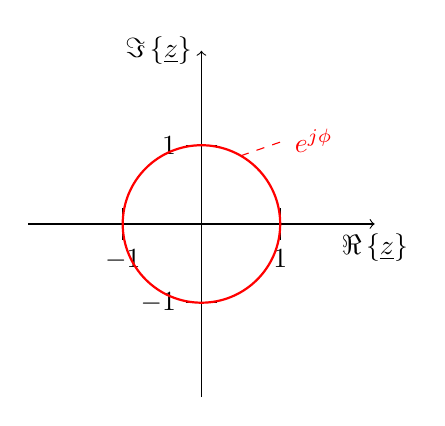
\begin{tikzpicture}
			\draw[->] (-2.2,0) -- (2.2,0) node[below, align=left]{$\Re\left\{\underline{z}\right\}$};
			\draw[->] (0,-2.2) -- (0,2.2) node[left, align=right]{$\Im\left\{\underline{z}\right\}$};
			%\draw (0:1) arc(0:360:1);
			\draw (1,0.2) -- (1,-0.2) node[below]{$1$};
			\draw (-1,0.2) -- (-1,-0.2) node[below]{$-1$};
			\draw (0.2,1) -- (-0.2,1) node[left]{$1$};
			\draw (0.2,-1) -- (-0.2,-1) node[left]{$-1$};
			
			\draw[thick, red] (0:1) arc(0:360:1);
			\draw[dashed, red] (60:1) -- (45:1.5) node[right, align=left, color=red]{$e^{j \phi}$};
		\end{tikzpicture}
		\caption{Complex plane of the complex frequency variable $\underline{z}$}
		\label{fig:ch04:ztrafo_z_cmplx_plane}
	\end{figure}
	
	In the \acf{DTFT}, $A = 1$ as a special case. The remainig $e^{j \phi}$ describes the unit circle in the complex plane. Like the Fourier transform, it assumes a steady-state, whereas the z-transform delivers a complete description of a time-discrete system. The z-transform is preferred for transient analysis of a time-discrete system. Its zeros $\underline{z}_0$ and poles $\underline{z}_\infty$ determine the stability of the system.
	
	\vspace{0.5em}
	
	Figure \ref{fig:ch04:ztrafo_z_cmplx_plane} makes evident the $2 \pi$-periodicity of both the \ac{DTFT} and z-transform. The frequency $e^{j \phi}$ repeats every $2 \pi$.
\end{excursus}

\subsubsection{Properties}

The \ac{DTFT} is derived from the \ac{CTFT}. Therefore, all properties apply likewise.
\begin{itemize}
	\item Linearity
	\item Time shift, frequency shift
	\item Convolution theorem
	\item Duality
	\item Symmetry rules
\end{itemize}

\subsection{Discrete Fourier Transform}

\subsubsection{Periodic Sequences}

Given is an $N$-periodic sequence of samples $\underline{x}_p[n]$:
\begin{equation}
	\underline{x}_p[n] = \underline{x}_p[n + mN] \qquad \forall \; m \in \mathbb{Z}
\end{equation}

A corollary of the periodicity is that the \ac{DTFT} $\underline{X}_{2 \pi} \left(e^{j \phi}\right)$ or $\underline{X}_{\frac{2\pi}{T_S}} \left(e^{j T_S \omega}\right)$, respectively, is not only periodic. It is zero for
\begin{itemize}
	\item $\underline{X}_{2 \pi} \left(e^{j \phi}\right) = 0$ for $\phi \neq m \frac{2\pi}{N}$ where $m \in \mathbb{Z}$, or
	\item $\underline{X}_{\frac{2\pi}{T_S}} \left(e^{j T_S \omega}\right) = 0$ for $\omega \neq m \frac{2\pi}{T_S N}$ where $m \in \mathbb{Z}$.
\end{itemize}
The \ac{DTFT} itself becomes a series of pulses (Dirac comb) with an equidistant spacing of
\begin{itemize}
	\item $\frac{2\pi}{N}$ for $\underline{X}_{2 \pi} \left(e^{j \phi}\right)$, or
	\item $\frac{2\pi}{T_S N}$ for $\underline{X}_{\frac{2\pi}{T_S}} \left(e^{j T_S \omega}\right)$, respectively.
\end{itemize}

This can be explained using the duality of the \ac{DTFT}:
\begin{figure}[H]
	\centering
	\begin{adjustbox}{scale=0.75}
		\begin{tikzpicture}
			\node[align=center, minimum width=2.5cm, minimum height=1.5cm] (TD1) {Sampled data is a Dirac comb\\ $\underline{x}_S(t) = \sum\limits_{n = -\infty}^{\infty} \underline{x}[n] \delta\left(t - n T_S\right)$};
			\node[align=center, minimum width=2.5cm, minimum height=1.5cm, right=3.5cm of TD1] (TD2) {Sampled data is periodic\\ $\underline{x}_S(t) = \underline{x}_S(t + m N {T_S})$};
			\node[align=center, minimum width=2.5cm, minimum height=1.5cm, below=2cm of TD1] (FD1) {Spectrum is periodic\\ $\underline{X}_{\frac{2\pi}{T_S}}(e^{j T_S \omega}) = \underline{X}_{\frac{2\pi}{T_S}}(e^{j T_S \left(\omega + \omega_S\right)})$};
			\node[align=center, minimum width=2.5cm, minimum height=1.5cm, below=2cm of TD2] (FD2) {Spectrum is a Dirac comb\\ $\underline{X}_{\frac{2\pi}{T_S}}(e^{j T_S \omega}) = \frac{1}{N} \sum\limits_{n = -\infty}^{\infty} \underline{X}[k] \delta\left(\omega - \frac{k}{N} \omega_S\right)$};
			
			\node[align=right, anchor=east, left=3cm of TD1] (LabelTD) {\textbf{Time domain}};
			\node[align=right, anchor=east, below=2cm of LabelTD] (LabelFD) {\textbf{Frequency domain}};
			\node[align=right, above=1cm of TD1] (Func1) {\textbf{Non-periodic function}};
			\node[align=right, above=1cm of TD2] (Func2) {\textbf{Periodic function}};
			
			%\draw (TD1) node[midway, align=right, rotate=-90]{$\TransformHoriz$} (FD1);
			%\draw (TD2) node[midway, align=right, rotate=-90]{$\TransformHoriz$} (FD2);
			\draw[o-*, thick] (TD1.south) -- (FD1.north);
			\draw[o-*, thick] (TD2.south) -- (FD2.north);
			
			\draw[thick] (TD1.south east) -- (FD2.north west);
			\draw[thick] (TD2.south west) -- (FD1.north east);
		\end{tikzpicture}
	\end{adjustbox}
	\caption{Due to the duality, the \ac{DTFT} of a periodic signal is series of pulses (Dirac comb).}
\end{figure}

The \ac{DTFT} of a periodic signal is still periodic. The maximum number of unique, discrete frequency samples in the \ac{DTFT} is
\begin{equation}
	\frac{\text{Periodicity of the \ac{DTFT}}}{\text{Spacing between the pulses}} = \frac{\frac{2\pi}{T_S}}{\frac{2\pi}{T_S N}} = N
\end{equation}

Because of the periodicity of both the time-domain and frequency-domain signal, the signal is fully determined by either
\begin{itemize}
	\item $N$ samples in the time domain, or
	\item $N$ samples in the frequency domain.
\end{itemize}

The samples in the frequency domain are
\begin{equation}
	\underline{X}[k] = \left.\underline{X}_{2 \pi} \left(e^{j \phi}\right)\right|_{\phi = k \frac{2\pi}{N}} = \left.\underline{X}_{\frac{2\pi}{T_S}} \left(e^{j T_S \omega}\right)\right|_{\omega = k \frac{2\pi}{T_S N}} = \sum\limits_{n = 0}^{N-1} \underline{x}[n] e^{-j 2\pi \frac{k}{N} n}
\end{equation}
where $k \in \mathbb{Z}$ is the discrete frequency variable. The summation boundaries $[0, N-1]$ can be replaced by any sequence of length $N$, because $\underline{x}[n]$ is $N$-periodic.

$\underline{X}[k]$ is the \ac{DFT}. $\underline{X}[k]$ is $N$-periodic.

The \ac{DTFT} is obtained by:
\begin{equation}
	\underline{X}_{\frac{2\pi}{T_S}} \left(e^{j T_S \omega}\right) = \frac{2\pi}{N T_S} \sum\limits_{k = -\infty}^{\infty} \underline{X}[k] \cdot \delta\left(\omega - \frac{k}{N} \underbrace{\frac{2\pi}{T_S}}_{= \omega_S}\right)
\end{equation}

\textit{Remark:} $\omega$ is normalized to $\frac{N T_S}{2\pi}$. Accordingly, the sum is normalized to $\frac{2\pi}{N T_S}$. Considerations analogous to the explanation on page \pageref{ref:ch04:normalization_xs} apply.

The inverse \ac{DTFT} is:
\begin{equation}
	\begin{split}
		\underline{x}[n] &= \frac{T_S}{2 \pi} \int\limits_{- \frac{\pi}{T_S}}^{+ \frac{\pi}{T_S}} \frac{2\pi}{N T_S} \sum\limits_{k = -\infty}^{\infty} \underline{X}[k] \cdot \delta\left(\omega - \frac{k}{N} \frac{2\pi}{T_S}\right) \cdot e^{+ j \omega T_S n} \, \mathrm{d} \omega \\
		 &\qquad \text{Integration boundaries propagate to summation boundaries via $\omega - \frac{k}{N} \frac{2\pi}{T_S} \stackrel{!}{=} 0$:} \\
		 &= \frac{1}{N} \sum\limits_{k = -\frac{N}{2}}^{\frac{N}{2}} \underline{X}[k] \cdot \int\limits_{- \frac{\pi}{T_S}}^{+ \frac{\pi}{T_S}} \delta\left(\omega - \frac{k}{N} \frac{2\pi}{T_S}\right) \cdot e^{+ j \omega T_S n} \, \mathrm{d} \omega \\
		 &\qquad \text{Using the Dirac measure:} \\
		 &= \frac{1}{N} \sum\limits_{k = -\frac{N}{2}}^{\frac{N}{2}} \underline{X}[k] \cdot e^{+ j 2\pi \frac{k}{N} n}
	\end{split}
\end{equation}
This is the inverse \ac{DFT}. Again the summation boundaries of $[-\frac{N}{2}, \frac{N}{2}]$ can be replaced by any sequence of length $N$, because $\underline{X}[k]$ is $N$-periodic.

\begin{definition}{Discrete Fourier transform}
	The \index{discrete Fourier transform} \textbf{\acf{DFT}} of a $N$-periodic sequence $\underline{x}[n]$ is:
	\begin{equation}
		\underline{X}[k] = \sum\limits_{n \in N} \underline{x}[n] \cdot e^{-j 2\pi \frac{k}{N} n}
	\end{equation}
	
	The \index{inverse discrete Fourier transform} \textbf{inverse discrete Fourier transform} is:
	\begin{equation}
		\underline{x}[n] = \frac{1}{N} \sum\limits_{k \in N} \underline{X}[k] \cdot e^{+ j 2\pi \frac{k}{N} n}
	\end{equation}
	
	Both $\underline{X}[k]$ and $\underline{x}[n]$ are $N$-periodic. The summation boundaries can be chosen to any sequence of length $N$.
\end{definition}

\subsubsection{Properties}

The \ac{DFT} is derived from the \ac{DTFT} and \ac{CTFT}. Therefore, all properties apply likewise.
\begin{itemize}
	\item Linearity
	\item Time shift, frequency shift
	\item Convolution theorem
	\item Duality
	\item Symmetry rules
\end{itemize}

\section{Analogies Of Time-Continuous and Time-Discrete Signals and Systems}

\subsection{Transforms}

\begin{table}[H]
	\centering
	\begin{tabular}{|p{0.3\linewidth}||p{0.3\linewidth}|p{0.3\linewidth}|}
		\hline
		{} & \textbf{Frequency-Continuous Domain} & \textbf{Frequency-Discrete Domain} \\
		\hline
		\hline
		\textbf{Time-Continuous Domain} & Fourier transform & Fourier series \\
		\hline
		\textbf{Time-Discrete Domain} & Discrete-Time Fourier transform & Discrete Fourier transform \\
		\hline
	\end{tabular}
\end{table}

\subsubsection{Obtaining a frequency-continuous domain:}

\begin{minipage}{0.45\linewidth}
	\textbf{From the time-continuous domain (analog signal):}
	
	\vspace{0.5em}
	
	Fourier transform:
	\begin{equation*}
		\underline{X}(j \omega) = \int\limits_{t = -\infty}^{\infty} \underline{x}(t) \cdot e^{-j \omega t} \, \mathrm{d} t
	\end{equation*}
	
	Inverse Fourier transform:
	\begin{equation*}
		\underline{x}(t) = \frac{1}{2 \pi} \int\limits_{\omega = -\infty}^{\infty} \underline{X}(j \omega) \cdot e^{+ j \omega t} \, \mathrm{d} \omega
	\end{equation*}
	
	\begin{itemize}
		\item Continuous time: $t \in \mathbb{R}$
		\item Continuous frequency: $\omega \in \mathbb{R}$
	\end{itemize}
\end{minipage}
\hfill
\begin{minipage}{0.45\linewidth}
	\textbf{From the time-discrete domain (digital signal):}
	
	\vspace{0.5em}
	
	Discrete-time Fourier transform:
	\begin{equation*}
		\underline{X}_{2\pi}(e^{j \phi}) = \sum\limits_{n = -\infty}^{\infty} \underline{x}[n] \cdot e^{- j \phi n}
	\end{equation*}
	
	Inverse discrete-time Fourier transform:
	\begin{equation*}
		\underline{x}[n] = \frac{1}{2 \pi} \int\limits_{- \pi}^{+ \pi} \underline{X}_{2\pi}(e^{j \phi}) \cdot e^{+ j \phi n} \, \mathrm{d} \phi
	\end{equation*}
	
	\begin{itemize}
		\item Discrete time: $n \in \mathbb{Z}$
		\item Continuous frequency: $\phi \in \mathbb{R}$
	\end{itemize}
\end{minipage}

\subsubsection{Obtaining a frequency-discrete domain:}

\begin{minipage}{0.45\linewidth}
	\textbf{From the time-continuous domain (analog signal):}
	
	\vspace{0.5em}
	
	Fourier analysis:
	\begin{equation*}
		\underline{X}[k] = \frac{\omega_0}{2 \pi} \int\limits_{-\frac{T_0}{2}}^{\frac{T_0}{2}} \underline{x}(t) \cdot e^{-j k \omega_0 t} \, \mathrm{d} t
	\end{equation*}
	
	Fourier series:
	\begin{equation*}
		\underline{x}(t) = \sum\limits_{k = -\infty}^{\infty} \underline{X}[k] \cdot e^{+ j k \omega_0 t}
	\end{equation*}
	
	\begin{itemize}
		\item Continuous time: $t \in \mathbb{R}$
		\item Discrete frequency: $k \in \mathbb{Z}$
	\end{itemize}
\end{minipage}
\hfill
\begin{minipage}{0.45\linewidth}
	\textbf{From the time-discrete domain (digital signal):}
	
	\vspace{0.5em}
	
	Discrete Fourier transform:
	\begin{equation*}
		\underline{X}[k] = \sum\limits_{n = 0}^{N - 1} \underline{x}[n] \cdot e^{- j \frac{2 \pi}{N} k n}
	\end{equation*}
	
	Inverse discrete Fourier transform:
	\begin{equation*}
		\underline{x}[n] = \frac{1}{N} \sum\limits_{k = 0}^{N - 1} \underline{X}[k]  \cdot e^{+ j \frac{2 \pi}{N} k n}
	\end{equation*}
	
	\begin{itemize}
		\item Discrete time: $n \in \mathbb{Z}$
		\item Discrete frequency: $k \in \mathbb{Z}$
	\end{itemize}
\end{minipage}

\subsection{Systems}

\subsection{Cross-Correlation and Autocorrelation}

\subsection{Spectral Density}

\subsection{Noise}

\section{Digital Signals and Systems}

\subsection{Quantization}

\subsection{Quantization Error}

\subsection{Window Filters}

\subsection{Time Recovery}

\subsection{Practical Issues}

\phantomsection
\addcontentsline{toc}{section}{References}
\printbibliography[heading=subbibliography]
\end{refsection}

